\documentclass[varwidth=true]{standalone}
\usepackage{tikz}
\begin{document}
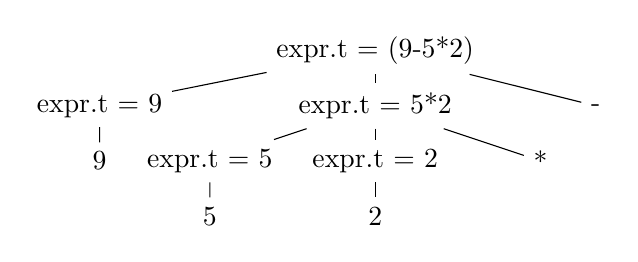
\begin{tikzpicture}[scale=0.7]
  \node (e) at (0, 0) {expr.t = (9-5*2)};

  \node (e9) at (-5, -1) {expr.t = 9};
  \node (e52) at (0, -1) {expr.t = 5*2};
  \node (-) at (4, -1) {-};
  \draw (e) -- (e9);
  \draw (e) -- (e52);
  \draw (e) -- (-);

  \node (9) at (-5, -2) {9};
  \draw (e9) -- (9);

  \node (e5) at (-3, -2) {expr.t = 5};
  \node (e2) at (0, -2) {expr.t = 2};
  \node (*) at (3, -2) {*};
  \draw (e52) -- (e5);
  \draw (e52) -- (e2);
  \draw (e52) -- (*);

  \node (5) at (-3, -3) {5};
  \draw (e5) -- (5);

  \node (2) at (0, -3) {2};
  \draw (e2) -- (2);
\end{tikzpicture}
\end{document}
